\documentclass{article}

\usepackage{verbatim}
\usepackage{tikz}
\usetikzlibrary{calc, backgrounds}

\title{Harmony Database Data Path}
\author{Cameron Kuchta}

\begin{document}
\maketitle

\section{Database Setup}

Both the rgt event and rgt check tables should be hardcoded into running. These will not be updated and instead only contain the information about what some event or exit status means.

\section{Action Times}

Updates to the database should occur whenever a test:
\begin{itemize}
	\item begins logging
	\item begins building
	\item finishes building
	\item starts running
	\item finishes running
	\item starts validating results
	\item finishes validating
\end{itemize}

We won't set up a push system but will instead look through the data files for updates and change the database according to those. We can do this for any time step but LSF is cleared once per hour. Thus, in order to get the correct exit status, we need to pull from LSF within that time period.

\section{When to Update}

Every $X$ seconds, we check the rgt master file. From this we get all of the tests that we may need to look into. We also want to look into all the tests that do not have a done flag on them.

\section{Updating}

Once we have decided that we want to check on some test, we need to check on all instances of that test that do not yet have a done flag attached to their entry. Since each test instance is labeled by it's harness uid, we can easily cross check this with the database. If the entry does not exist then we need to create such an entry. We wait to do this until we have begun logging the test.

\subsection{Beginning to Log}

We find if a test has begun logging once the Event 110 file occurs in the test directory. Once this file is created, we parse it into a dictionary. From this we can easily find the necessary information for the \texttt{rgt\_test} table. 
Namely,
\begin{itemize}
	\item Test ID
	\item Harness start time
	\item App name
	\item Test name
	\item System
	\item Harness tld (path to where the test is stored)
\end{itemize}

We also create an event in the \texttt{rgt\_test\_event} table that is associated with this harness uid labeling it as beginning to run.

\subsection{Events}

When a new event file appears, we create the corresponding event in \texttt{rgt\_test\_event} and change the corresponding status. If it is beginning, we must decide some number for what it means to be currently running. If it is ending, the event status is entered into the table as well.

We always need to check the LSF status of the job once it has begun running. This is because the system may have caused an error that forced the test to interrupt before creating any event files. If it is still running, there is nothing to worry about. If it indeed has been exited for some reason, we record this exit status. We also need to make sure that the next test knows what lsf job to check on while it is building. This is because the next test is built at the end of the current tests run. It is somewhat difficult to correlate the exit status with the an actual problem with the test because it may be due to the test or the test that it is building for the next run or just a system error.

\newpage

\section{State Machine}

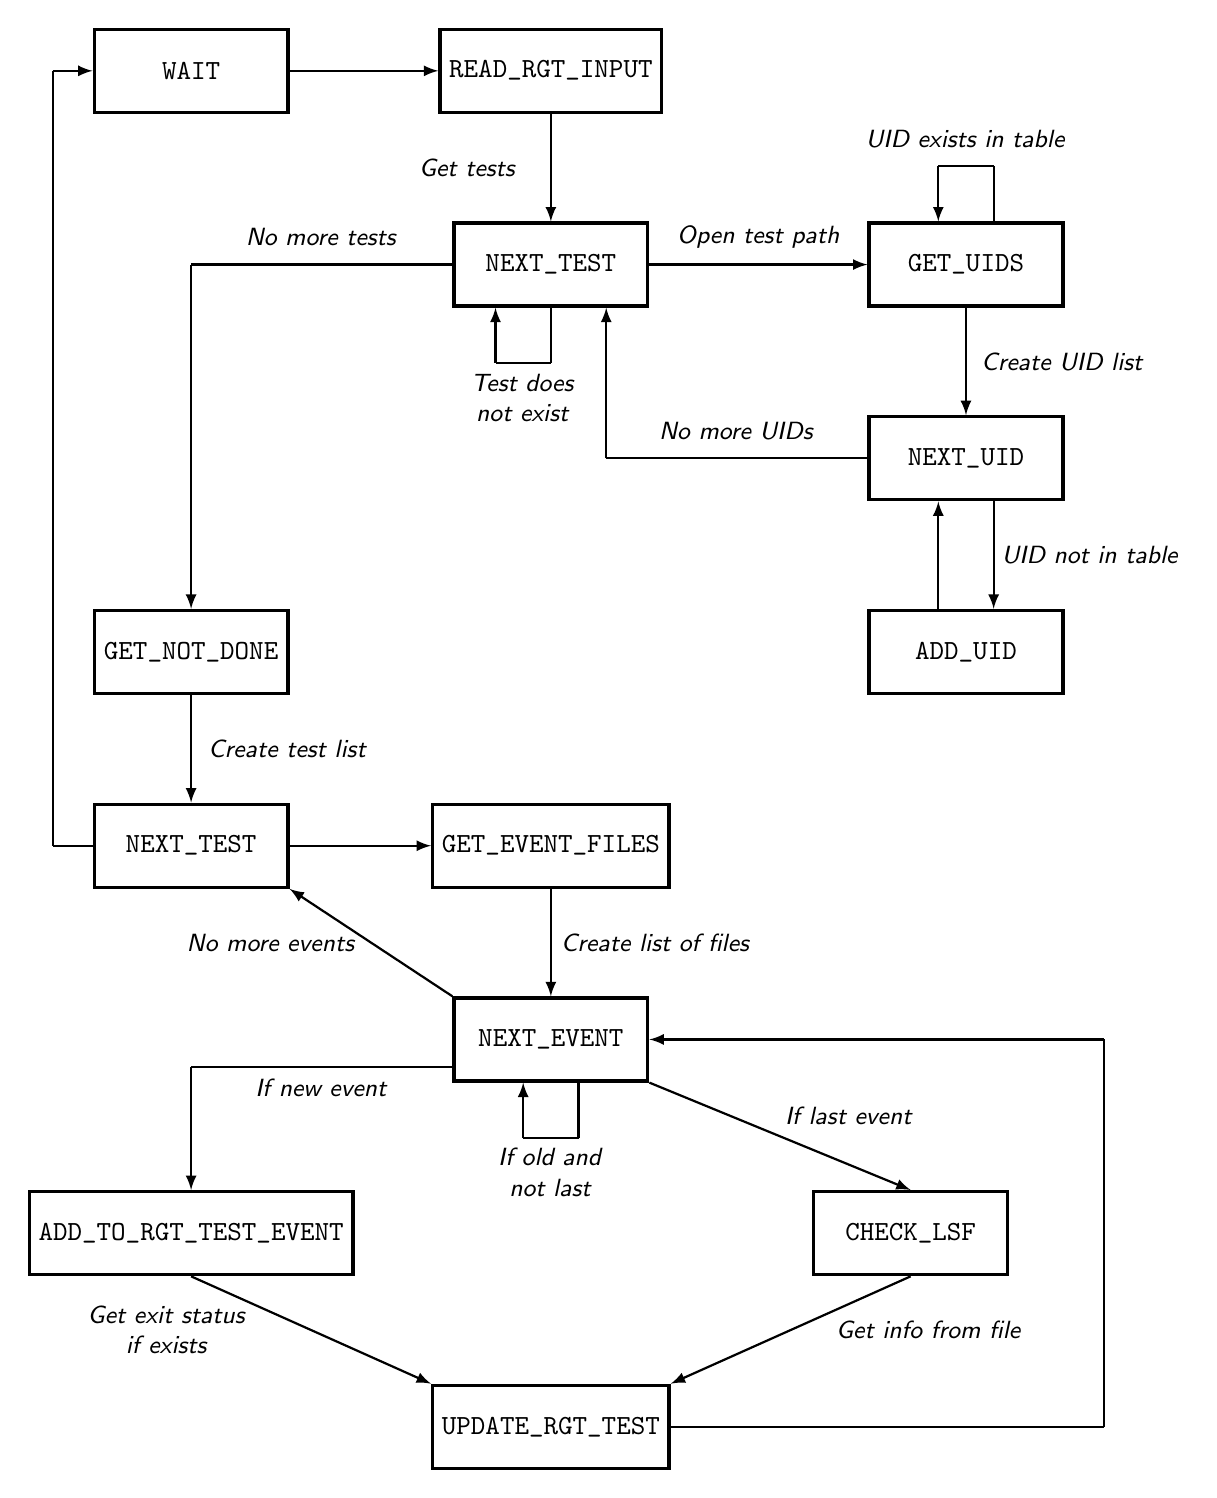
\begin{tikzpicture}[>=latex]

  %
  % Styles for states, and state edges
  %
  \tikzstyle{state} = [draw, very thick, fill=white, rectangle, minimum height=3em, minimum width=7em, node distance=7em, font={\ttfamily}]
  \tikzstyle{stateEdgePortion} = [black,thick];
  \tikzstyle{stateEdge} = [stateEdgePortion,->];
  \tikzstyle{edgeLabel} = [pos=0.5, text centered, font={\sffamily\small}];

  %
  % Position States
  % wait_time, read database and paths for rgt, get all not done database entries and all tests in path with uid that are not in database, add new uid to database
  % for each test, for each event, test if event exists in db, if not then add to db and change status of corresponding val, wait

  \node[state, name=readRGTInput] {READ\char`_RGT\char`_INPUT};
  \node[state, name=wait, left of=readRGTInput, xshift=-6em] {WAIT};
  \node[state, name=nextTest, below of=readRGTInput] {NEXT\char`_TEST};
  \node[state, name=getUIDs, right of=nextTest, xshift=8em] {GET\char`_UIDS};
  \node[state, name=nextUID, below of=getUIDs] {NEXT\char`_UID};
  \node[state, name=addUID, below of=nextUID] {ADD\char`_UID};

  \node[state, name=getNotDone, left of=addUID, xshift=-21em] {GET\char`_NOT\char`_DONE};
  \node[state, name=nextTestA, below of=getNotDone] {NEXT\char`_TEST};
  \node[state, name=getEventFiles, right of=nextTestA, xshift=6em] {GET\char`_EVENT\char`_FILES};
  \node[state, name=nextEvent, below of=getEventFiles] {NEXT\char`_EVENT};
  \node[state, name=addToRGTTestEvent, below of=nextEvent, left of=nextEvent, xshift=-6em] {ADD\char`_TO\char`_RGT\char`_TEST\char`_EVENT};
  \node[state, name=checkLSF, below of=nextEvent, right of=nextEvent, xshift=6em] {CHECK\char`_LSF};
  \node[state, name=updateRGTTest, below of=nextEvent, yshift=-7em] {UPDATE\char`_RGT\char`_TEST};

  % Draw edges between states

  \draw (wait.east)
      edge[stateEdge]
      (readRGTInput.west);

  \draw (readRGTInput.south) 
      edge[stateEdge] node[edgeLabel, xshift=-3em]{\emph{Get tests}} 
      (nextTest.north); 

  \draw (nextTest.east) 
      edge[stateEdge] node[edgeLabel, xshift=0em, yshift=1em]{\emph{Open test path}} 
      (getUIDs.west); 

  \draw (getUIDs.south) 
      edge[stateEdge] node[edgeLabel, xshift=3.5em]{\emph{Create UID list}} 
      (nextUID.north); 

  \draw ($(nextUID.south) + (1em, 0)$) 
      edge[stateEdge] node[edgeLabel, xshift=3.5em]{\emph{UID not in table}} 
      ($(addUID.north) + (1em, 0)$); 

  \draw ($(addUID.north) + (-1em, 0)$) 
      edge[stateEdge] 
      ($(nextUID.south) + (-1em, 0)$); 

  \path let \p1=(nextTest.south), \p2=(nextUID) in coordinate (nextUID2nextTestA) at (\x1 + 2em, \y2);

  \draw (nextUID)
  	  edge[stateEdgePortion] node[edgeLabel, yshift=1em]{\emph{No more UIDs}} 
  	  (nextUID2nextTestA);

  \draw (nextUID2nextTestA)
      edge[stateEdge]
      ($(nextTest.south) + (2em, 0)$);

  \coordinate (getUIDs2getUIDSA) at ($(getUIDs.north) + (1em, 2em)$);
  \coordinate (getUIDs2getUIDSB) at ($(getUIDs2getUIDSA) + (-2em, 0em)$);
  \coordinate (getUIDs2getUIDSC) at ($(getUIDs2getUIDSB) + (0em, -2em)$);

  \draw ($(getUIDs.north) + (1em, 0)$)
      edge[stateEdgePortion]
      (getUIDs2getUIDSA);

  \draw (getUIDs2getUIDSA)
      edge[stateEdgePortion] node[edgeLabel, yshift=1em] {\emph{UID exists in table}}
      (getUIDs2getUIDSB);

  \draw (getUIDs2getUIDSB)
      edge[stateEdge]
      (getUIDs2getUIDSC);

  \coordinate (nextTest2nextTestA) at ($(nextTest.south) + (0, -2em)$);
  \coordinate (nextTest2nextTestB) at ($(nextTest2nextTestA) + (-2em, 0em)$);
  \coordinate (nextTest2nextTestC) at ($(nextTest2nextTestB) + (0em, 2em)$);

  \draw (nextTest.south)
      edge[stateEdgePortion]
      (nextTest2nextTestA);

  \draw (nextTest2nextTestA)
      edge[stateEdgePortion] node[edgeLabel, yshift=-1.25em, align=center] {\emph{Test does} \\ \emph{not exist}}
      (nextTest2nextTestB);

  \draw (nextTest2nextTestB)
      edge[stateEdge]
      (nextTest2nextTestC);

  \path let \p1=(getNotDone), \p2=(nextTest) in coordinate (nextTest2getNotDoneA) at (\x1, \y2);

  \draw (nextTest.west)
      edge[stateEdgePortion] node[edgeLabel, yshift=1em]{\emph{No more tests}}
      (nextTest2getNotDoneA);

  \draw (nextTest2getNotDoneA)
  	  edge[stateEdge]
  	  (getNotDone.north);

  \draw (getNotDone.south)
      edge[stateEdge] node[edgeLabel, xshift=3.5em, yshift=0em]{\emph{Create test list}}
      (nextTestA.north);

  \draw (nextTestA.east)
      edge[stateEdge]
      (getEventFiles.west);

  \draw (getEventFiles.south)
  	  edge[stateEdge] node[edgeLabel, xshift=3.8em]{\emph{Create list of files}}
  	  (nextEvent.north);

  \draw (nextEvent.north west)
  	  edge[stateEdge] node[edgeLabel, xshift=-3.6em]{\emph{No more events}}
  	  (nextTestA.south east);


  \coordinate (nextEvent2nextEventA) at ($(nextEvent.south) + (1em, -2em)$);
  \coordinate (nextEvent2nextEventB) at ($(nextEvent2nextEventA) + (-2em, 0em)$);
  \coordinate (nextEvent2nextEventC) at ($(nextEvent2nextEventB) + (0em, 2em)$);

  \draw ($(nextEvent.south) + (1em,0)$)
      edge[stateEdgePortion]
      (nextEvent2nextEventA);

  \draw (nextEvent2nextEventA)
      edge[stateEdgePortion] node[edgeLabel, yshift=-1.25em, align=center] {\emph{If old and} \\ \emph{not last}}
      (nextEvent2nextEventB);

  \draw (nextEvent2nextEventB)
      edge[stateEdge]
      (nextEvent2nextEventC);


  \path let \p1=(addToRGTTestEvent), \p2=(nextEvent) in coordinate (nextEvent2addToRGTTestEvent) at (\x1, \y2 - 1em);

  \draw ($(nextEvent.west) + (0,-1em)$)
  	  edge[stateEdgePortion] node[edgeLabel, yshift=-0.75em]{\emph{If new event}}
  	  (nextEvent2addToRGTTestEvent);

  \draw (nextEvent2addToRGTTestEvent)
  	  edge[stateEdge]
  	  (addToRGTTestEvent.north);

  \draw (nextEvent.south east)
      edge[stateEdge] node[edgeLabel, xshift=2.5em, yshift=0.75em]{\emph{If last event}}
      (checkLSF.north);

  \draw (checkLSF.south)
      edge[stateEdge] node[edgeLabel, xshift=5em, yshift=0em]{\emph{Get info from file}}
      (updateRGTTest.north east);

  \draw (addToRGTTestEvent.south)
      edge[stateEdge] node[edgeLabel, xshift=-5.2em, yshift=0em, align=center]{\emph{Get exit status} \\ \emph{if exists}}
      (updateRGTTest.north west);

  \coordinate (updateRGTTest2nextEventA) at ($(updateRGTTest) + (20em,0)$);
  \coordinate (updateRGTTest2nextEventB) at ($(nextEvent) + (20em,0)$);

  \draw (updateRGTTest.east)
      edge[stateEdgePortion]
      (updateRGTTest2nextEventA);

  \draw (updateRGTTest2nextEventA)
      edge[stateEdgePortion]
      (updateRGTTest2nextEventB);

  \draw (updateRGTTest2nextEventB)
      edge[stateEdge]
      (nextEvent.east);

  \coordinate (nextTestA2waitA) at ($(nextTestA) + (-5em,0)$);
  \coordinate (nextTestA2waitB) at ($(wait) + (-5em,0)$);

  \draw (nextTestA.west)
      edge[stateEdgePortion]
      (nextTestA2waitA);

  \draw (nextTestA2waitA)
      edge[stateEdgePortion]
      (nextTestA2waitB);

  \draw (nextTestA2waitB)
      edge[stateEdge]
      (wait.west);
\end{tikzpicture}

\end{document}